\documentclass[12pt,a4paper]{article}
%\usepackage{ctex}
\usepackage{amsmath,amscd,amsbsy,amssymb,latexsym,url,bm,amsthm}
\usepackage{epsfig,graphicx,subfigure}
\usepackage{enumitem,balance}
\usepackage{wrapfig}
\usepackage{mathrsfs,euscript}
\usepackage[x11names,svgnames,dvipsnames]{xcolor}
\usepackage{hyperref}
\usepackage[vlined,ruled,commentsnumbered,linesnumbered]{algorithm2e}
\usepackage{listings}
%\usepackage{fontspec}

\newtheorem{theorem}{Theorem}
\newtheorem{lemma}[theorem]{Lemma}
\newtheorem{proposition}[theorem]{Proposition}
\newtheorem{corollary}[theorem]{Corollary}
\newtheorem{exercise}{Exercise}
\newtheorem*{solution}{Solution}
\newtheorem{definition}{Definition}
\theoremstyle{definition}


%\numberwithin{equation}{section}
%\numberwithin{figure}{section}

\renewcommand{\thefootnote}{\fnsymbol{footnote}}

\newcommand{\postscript}[2]
 {\setlength{\epsfxsize}{#2\hsize}
  \centerline{\epsfbox{#1}}}

\renewcommand{\baselinestretch}{1.0}

\setlength{\oddsidemargin}{-0.365in}
\setlength{\evensidemargin}{-0.365in}
\setlength{\topmargin}{-0.3in}
\setlength{\headheight}{0in}
\setlength{\headsep}{0in}
\setlength{\textheight}{10.1in}
\setlength{\textwidth}{7in}
\makeatletter \renewenvironment{proof}[1][Proof] {\par\pushQED{\qed}\normalfont\topsep6\p@\@plus6\p@\relax\trivlist\item[\hskip\labelsep\bfseries#1\@addpunct{.}]\ignorespaces}{\popQED\endtrivlist\@endpefalse} \makeatother
\makeatletter
\renewenvironment{solution}[1][Solution] {\par\pushQED{\qed}\normalfont\topsep6\p@\@plus6\p@\relax\trivlist\item[\hskip\labelsep\bfseries#1\@addpunct{.}]\ignorespaces}{\popQED\endtrivlist\@endpefalse} \makeatother


\definecolor{codegreen}{rgb}{0.44,0.68,0.28}
\definecolor{codegray}{rgb}{0.5,0.5,0.5}
\definecolor{codepurple}{rgb}{0.58,0,0.82}
\definecolor{backcolour}{rgb}{0.96,0.96,0.96}

\lstset{ 
language=C++, 
frame=shadowbox,
keywordstyle = \color{blue}\bfseries, 
commentstyle=\color{codegreen}, 
tabsize = 4, 
backgroundcolor=\color{backcolour}, 
numbers=left,                    
numbersep=5pt,
breaklines=true, 
escapechar=|,
emph = {int,float,double,char},emphstyle=\color{orange}, 
emph ={[2]const, typedef},emphstyle = {[2]\color{red}} } 


 
\begin{document}
\noindent

%========================================================================
\noindent\framebox[\linewidth]{\shortstack[c]{
\Large{\textbf{Lab01-Preliminary}}\vspace{1mm}\\
VE281 - Data Structures and Algorithms, Xiaofeng Gao, TA: Qingmin Liu, Autumn 2019}}
%CS26019 - Algorithm Design and Analysis, Xiaofeng Gao, Autumn 2019}}
\begin{center}
\footnotesize{\color{red}$*$ Please upload your assignment to website. Contact webmaster for any questions.}

\footnotesize{\color{blue}$*$ Name: Sun Yiwen  \quad Student ID: 517370910213 \quad Email: sunyw99@sjtu.edu.cn}
\end{center}


\begin{enumerate}

\item What is the time complexity of the following code?


\begin{lstlisting}[language=C++]
// REQUIRES: an integer k
// EFFECTS: return the number of times that Line|\color{codegreen}~\ref{Line-Count}| is executed
int count(int k)
{
	int count = 0;
	int n = pow(2,k); // n=2^k
	while (n>=1)
	{
		int j;
   		for (j=0;j<n;j++)
   		{
   			count += 1;  |\label{Line-Count}|	
   		}
   		n /= 2;
	}
	return count;
}
\end{lstlisting}



\begin{solution}
The statements \textbf{j$<$n;} \textbf{j++;} \textbf{count+=1;} all occur $2^k+2^{k+1}+...+2+1$ times.
Suppose $T(k)=2^k+2^{k+1}+...+2+1$, then if we pick constants $c$ and $k_0$ so that for any $k>k_0$, $T(k)\leq c\cdot 2^k$, then we can prove $T(k)=O(2^k)$.
We choose $c=2$ and $k_0=1$, then for any $k>1$, $T(k)=2^k+2^{k+1}+...+2+1<2^k+2^{k+1}+...+2+1+1=2^{k+1}=2\cdot 2^k$.
Therefore, the time complexity of the above code is $O(2^k)$.
\end{solution}


\item Given an array \textbf{nums} of $n$ integers, are there elements $a, b, c$ in nums such that $a + b + c = 0?$ Write a program to find all unique triplets in the array which gives the sum of zero. Give your code as the answer. \textbf{Claim that the time complexity of your program should be less than or equal to $O(n^2)$.}

{\color{purple}Examples: Input array [-1, 0, 1, 2, -1, -4], the solution is [[-1, 0, 1], [-1, -1, 2]]}



\begin{solution}
Please explain your design and fill in the following block:
%vector<vector<int>> findTriplet(vector<int>& nums, int n)
{
	vector<vector<int>> res;
	int i=0, j=0, k=n-1;
	for (i=0;i<n-2;i++)
	{
		TODO
	}
	return res;
}%
	\begin{lstlisting}[language=C++]
// REQUIRES: an integer array nums of size n
// EFFECTS: return a list of triplets, the sum of each triplet equals to 0.
#include <vector>
vector<vector<int>> findTriplet(vector<int>& nums, int n)
{
	vector<vector<int>> res;
	vector<int> ans;
	vector<int> sorted;
	int i, j, k;
	for (i = 0; i < n; i++) {
		if (sorted.empty()) sorted.push_back(nums[0]);
		else {
			vector<int>::iterator it;
			for (it = sorted.begin(); it != sorted.end(); ++it) {
				if (nums[i] <= *it) {
					sorted.insert(it, nums[i]);
					break;
				}
				else if (it == sorted.end() - 1) {
					sorted.push_back(nums[i]);
					break;
				}
			}
		}
	}
	for (i = 0; i < n - 2; i++) {
		while (i > 0 && sorted[i] == sorted[i - 1]) i++;
		j = i + 1;
		k = n - 1;
		while (j < k) {
			if (sorted[i] + sorted[j] + sorted[k] < 0) j++;
			else if (sorted[i] + sorted[j] + sorted[k] > 0) k--;
			else {
				ans.push_back(sorted[i]);
				ans.push_back(sorted[j]);
				ans.push_back(sorted[k]);
				if (res.empty()) res.push_back(ans);
				else if (ans != res.back()) res.push_back(ans);
				ans.clear();
				j++;
			}
		}
	}
	return res;
}
	\end{lstlisting}
Explain the time complexity of your solution here.\\
My code can be divided into two parts. The first part(ll.10-25) is where the program sorts the original array in ascending order, which is necessary because we want all the triplets in the result to be unique. The second part(ll.26-43) is where the program finds all unique triplets that meet the requirement.\\
For the first part, note that the statements \textbf{i$<$n;} \textbf{i++;} \textbf{if (sorted.empty())...else...} all occur $n$ times. The time complexity can be calculated as $O(n)$. For the second part, note that the statements \textbf{j$<$k;} occur $(n-1)+(n-2)+...+2=\dfrac{(n-1+2)(n-2)}{2}$ times in the worst case. So the time complexity of the second part can be calculated as $O(n^2)$. Because of the rule that “If $f_1(n)=O(g_1(n))$ and $f_2(n)=O(g_2(n))$, then $f_1(n)+f_2(n)=O(max\{g_1(n),g_2(n)\})$", the time complexity of my entire solution is $O(n^2)$.
\end{solution}

\item Equivalence Class

\begin{definition}[$o$-Notation]
Let $f(n)$ and $g(n)$ be functions from the set of natural numbers to the set of nonnegative real numbers. $f(n)$ is said to be $o(g(n))$, written as $f(n)=o(g(n))$, if
$$\forall c.\exists n_{0}.\forall n\ge n_{0}.f(n)<c g(n).$$
\end{definition}

An equivalence relation $\mathcal{R}$ on the set of complexity functions is defined as follows: $$f\mathcal{R}g \mbox{ if and only if }
f(n)=\Theta(g(n)).$$ A complexity class is an equivalence class of $\mathcal{R}$.

The equivalence classes can be ordered by $\prec$ defined as: $f\prec g$ iff $f(n)=o(g(n))$.

{\color{purple}Example: $1 \prec \log \log n \prec \log n \prec \sqrt{n} \prec n^{\frac{3}{4}} \prec n \prec n \log n \prec n^2 \prec 2^n \prec n! \prec 2^{n^2}$.}

Please order the following functions by $\prec$ and give your explanation: $$(\sqrt{2})^{\log n}, (n+1)!, 
ne^n, (\log n)!, n^3,  n^{1/\log n}.$$




\begin{solution}
\begin{enumerate}
\item
Using the formula $a^{log_{b}c}=c^{log_{b}a}$, we can get $(\sqrt{2})^{\log n}=n^{log\sqrt{2}}=n^{1/2}=\sqrt{n}$.
\item
Since $(n+1)!-n!=n+1$, we get $n! < (n+1)!$ for $n\geq 1$. With $n$ approaching infinity, $(n+1)!\rightarrow n!$. Therefore, $n! \prec (n+1)!$
\item
Since $e>2$, for $n\geq 1$, $e^n>2^n$. Since $ne^n-e^n=(n-1)e^n$, we get $ne^n>e^n$ for $n>1$. Therefore, $2^n\prec ne^n$.\\
We want to show $\lim_{n\rightarrow\infty}\dfrac{ne^n}{n!}=0$. Let $n>2e$.\\
$\dfrac{ne^n}{n!}=\dfrac{e^{n-2e}a^{2e}}{(n-1)(n-2)...(2e)(2e-1)!}<\dfrac{e^{n-2e}e^{2e}}{n^{n-2e}(2e-1)!}<\left(\dfrac{1}{2}\right)^{n-2e}\dfrac{e^{2e}}{(2e-1)!}$\\
$\dfrac{e^{2e}}{(2e-1)!}$ is constant, $\left(\dfrac{1}{2}\right)^{n-2e}\rightarrow 0$ as $n\rightarrow\infty$.\\
Therefore, $ne^n\prec n!$.
\item
According to the Stirling's approximation, the most important term of the Stirling's approximation of the factorial is $n^n$. So $(\log n)!$ can be approximated as $\log n^{\log n}$, with some extra factors which make it a bit smaller.\\
$\log n^{\log n}=e^{\log\log n\cdot\log n}=e^{\log n\cdot\log\log n}=n^{\log \log n}$.\\
Since $\log \log n \prec \log n \prec \sqrt{n}$, we get $\log \log n \cdot \log n \prec \sqrt{n}\cdot\sqrt{n}=n$. Thus, as $n$ approaches infinity, $e^{\log \log n \cdot \log n}<e^n$.\\
Therefore, $(\log n)!\prec e^n$.\\
$f(n)=\log\log n$ is monotonically increasing and $f(500)=\log\log 500\approx3.164>3$. Thus, as $n\rightarrow\infty$, $\log\log n>3$. And we get $\lim_{n\rightarrow\infty}\dfrac{n^3}{n^{\log\log n}}=0$.\\
Therefore, $n^3\prec(\log n)!$.\\
\item
$f(n)=\log n$ is monotonically increasing and $f(4)=\log 4=2$. Thus, for $n>4$, $\log n>2\Rightarrow\dfrac{1}{\log n}<\dfrac{1}{2}\Rightarrow n^{1/\log n}<n^{1/2}$. Therefore, $n^{1/\log n}\prec\sqrt{n}$.
\end{enumerate}
Combining all the above with the given Example, we get the final result:$$n^{1/\log n}\prec(\sqrt{2})^{\log n}\prec n^3\prec (\log n)!\prec ne^n\prec (n+1)!$$
Now, I would like to plot graphs using Wolfram Mathematica to further prove my result.
The Mathematica code are as follows:\\
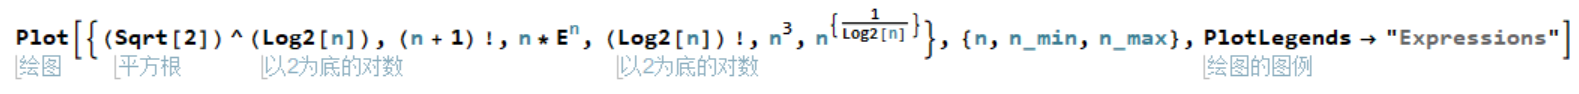
\includegraphics[width=0.9\textwidth]{f_1.png}\\
Note that $n_{min}$ and $n_{max}$ will be replaced with actual numbers to change the scale when plotting. The following graphs are the plot results when the scale is $n\in[0,500]$, $n\in[0,1000]$, $n\in[0,1000000]$, $n\in[2,2.7]$ correspondingly.\\
\begin{figure}[htbp]
\begin{minipage}[h]{0.5\textwidth}
\centering
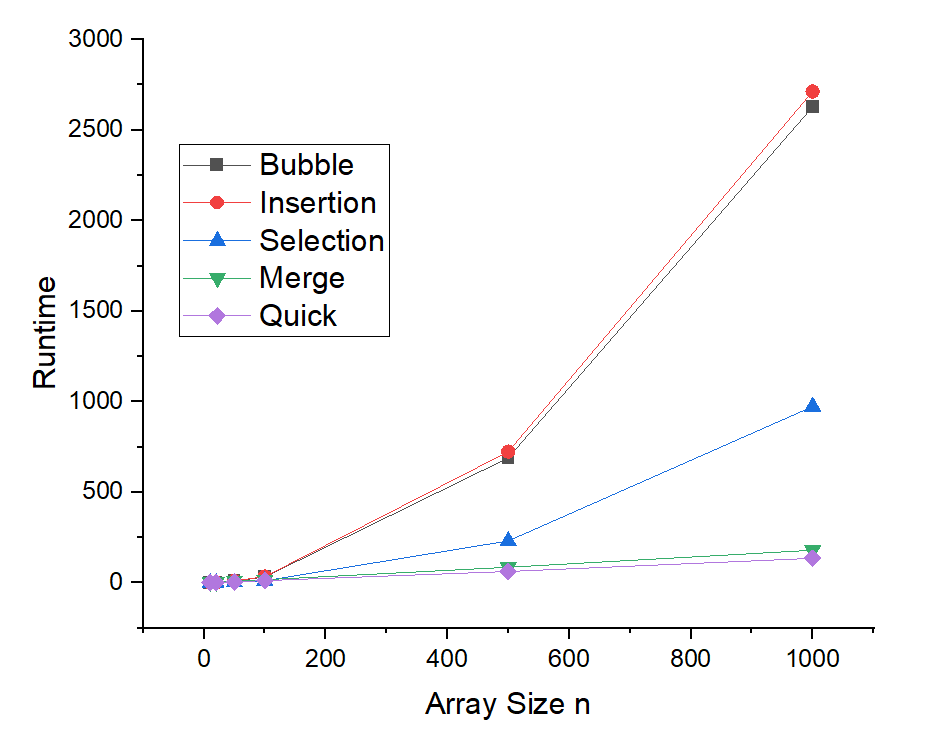
\includegraphics[width=1\textwidth]{f1.png}
\caption{Function plots when $n\in[0,500]$.} 
\end{minipage}
\begin{minipage}[h]{0.5\textwidth}
\centering
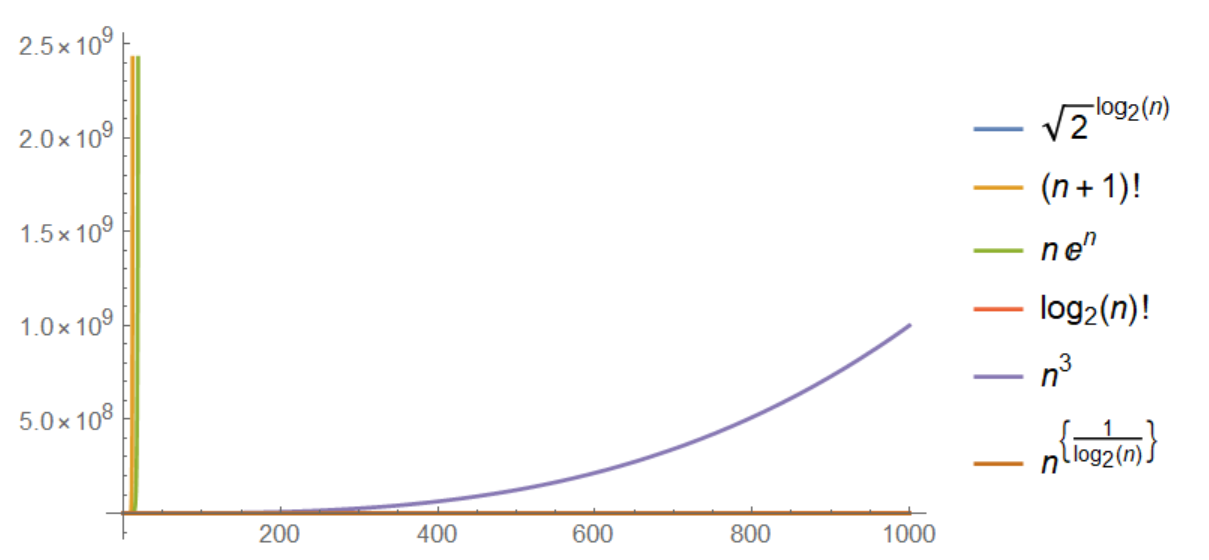
\includegraphics[width=1\textwidth]{f2.png}
\caption{Function plots when $n\in[0,1000]$.} 
\end{minipage}
\end{figure}

\begin{figure}[htbp]
\begin{minipage}[h]{0.5\textwidth}
\centering
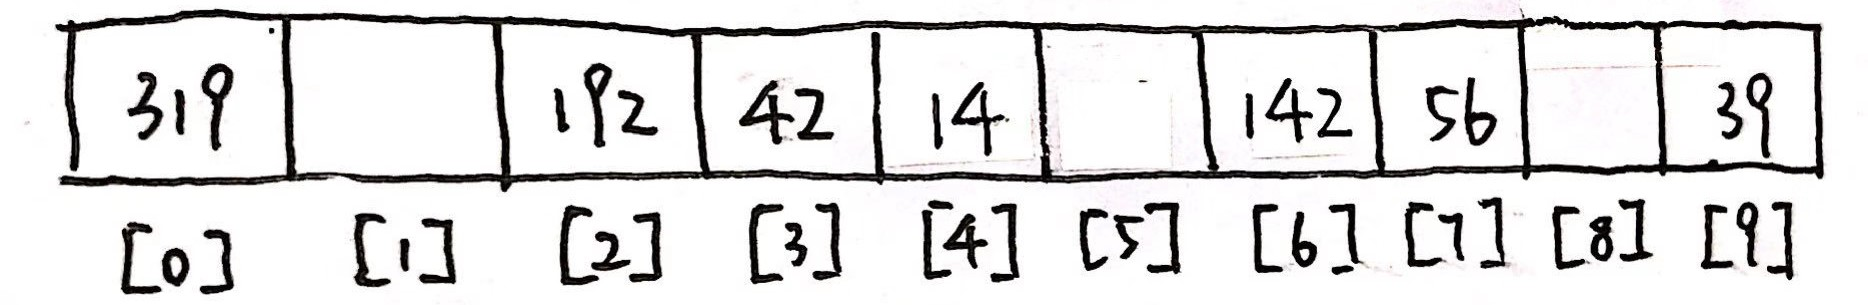
\includegraphics[width=1\textwidth]{f3.png}
\caption{Function plots when $n\in[0,1000000]$.} 
\end{minipage}
\begin{minipage}[h]{0.5\textwidth}
\centering
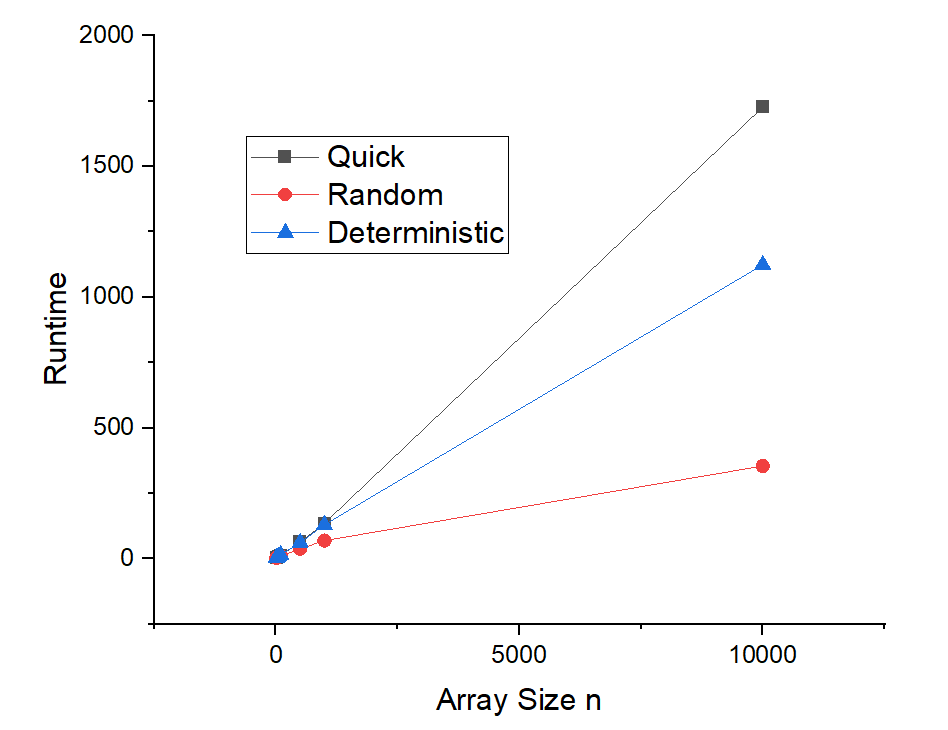
\includegraphics[width=1\textwidth]{f4.png}
\caption{Function plots when $n\in[2,2.7]$.} 
\end{minipage}
\end{figure}
As shown in Figure 1 and Figure 2, the growing rate of $(n+1)!$ is greater than $ne^n$ and the growing rate of $(n+1)!$ and $ne^n$ are greater than the other four functions. Although $(\log n)!$ seems to grow slower than $n^3$ in Figure 2, according to Figure 3, it will catch up with and eventually surpass $n^3$ around $n=600000$. As shown in Figure 3, $n^{1/\log n}$ and $(\sqrt{2})^{\log n}$ grow much slower than the other four functions. And according to Figure 4, the growing rate of $(\sqrt{2})^{\log n}$ is a little bit faster than $n^{1/\log n}$.\\
In conclusion, we get the same result:
$$n^{1/\log n}\prec(\sqrt{2})^{\log n}\prec n^3\prec (\log n)!\prec ne^n\prec (n+1)!$$
Again, we cannot assume these four plots give us the correct result for they only show us parts of the functions. But they can be back-up evidence for my mathematical proof in the previous part.
\end{solution}

\end{enumerate}

%========================================================================
\end{document}
